\section{\peregrine: Efficiently Enforcing Schedules} \label{sec:peregrine}

%% challenge 1: dmt race \vs overhead
%% challenge 2: manual annotation
%% insight: can detect race, and compute precond, detect races in memoized
%%          schedules, and enforce races later.
%% key idea of the slicing algorithm
%% results: overhead

Prior work enforces schedules at two different granularities: shared
memory accesses or synchronizations, forcing users to trade off efficiency
and determinism.  Specifically, memory access schedules make data races
deterministic but are prohibitively inefficient (\eg, 1.2X-6X as slow as
traditional multithreading~\cite{coredet:asplos10}); synchronization
schedules are much more efficient (\eg, average 16\%
slowdown~\cite{kendo:asplos09}) because they are coarse grained, but they
cannot make programs with data races deterministic~\cite{lu:concurrency-bugs,syncfinder:osdi10}.
This determinism \vs performance challenge has been open for decades in the areas of
deterministic execution and replay.  Because of this challenge, 
\tern, our first \smt system, enforces only synchronization schedules.

To address this challenge, we have built \peregrine, our second \smt
system~\cite{peregrine:sosp11}.  The insight in \peregrine is that although
many programs have races, the races tend to occur only within small
portions of an execution, and the majority of the execution is still
race-free.  Intuitively, if a program is full of data races, most of them
would have been caught during testing.  Empirically, we analyzed the
executions of seven real programs with races, and found that, despite
millions of memory accesses, only up to 10 data races were detected per
execution.

Since races occur rarely, we can schedule synchronizations for the
race-free portions of an execution, and resort to scheduling memory
accesses only for the ``racy'' portions, combining both the efficiency of
synchronization schedules and the determinism of memory access schedules.
These hybrid schedules are almost as coarse-grained as synchronization
schedules, so they can also be frequently reused.  
Figure~\ref{fig:hybrid-schedule} illustrates this idea.

How can we predict where data races may occur before an execution actually
starts?  One possible idea is to use static analysis to detect data races
at compile time.
%  and treat the offending load and store instructions as synchronizations.
However, static race detectors are notoriously imprecise: a majority of
their reports tend to be false reports, not true data races.  Scheduling
many memory accesses in the false reports would severely slow down the
execution.

\begin{figure}[t]
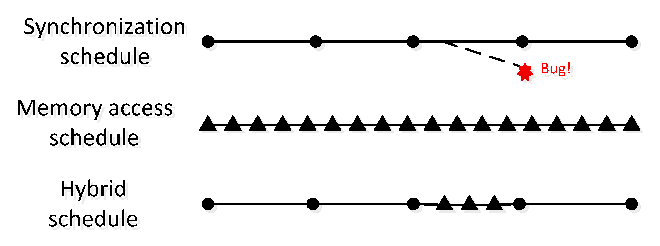
\includegraphics[width=0.7\linewidth]{peregrine/figures/hybrid-schedule}
\caption{{\em Hybrid schedule idea.} Circles represent synchronizations,
  and triangles memory accesses.  A synchronization schedule is efficient
  because it is coarse-grained, but it is not deterministic because data
  races may still cause executions to deviate from the schedule and
  fail.  A memory access schedule is
  deterministic, but it is slow because it is fine-grained.  A hybrid
  schedule combines the best of both by scheduling memory access only for
  the racy portion of an execution and synchronizations
  otherwise.} \label{fig:hybrid-schedule}
\end{figure}


\peregrine leverages the record-and-reuse approach in \tern to predict races:
a recorded execution can effectively foretell what may happen for
executions reusing the same schedule.  Specifically, when recording a
synchronization schedule, \peregrine records a detailed memory access trace.
From the trace, it detects data races that occurred (with respect to the
schedule), and adds the memory accesses involved in the races to the
schedule.  Now, this hybrid schedule can be efficiently and
deterministically enforced, solving the aforementioned open challenge.
To reuse the schedule on other inputs, \peregrine provides new precondition
computation algorithms to guarantee that executions reusing the schedule
will not run into any new data races. To enforce an order on memory
accesses, \peregrine modifies a live program at runtime using
a safe, efficient instrumentation framework we built~\cite{wu:loom:osdi10}.

Server programs present three challenges for \smt. First, they may run
continuously, making their schedules effectively infinite and too specific
to reuse.  Second, they often process inputs, \ie, client requests, as
soon as the requests arrive. Each request may arrive at a random moment,
causing a different schedule. Third, since requests do not arrive at the
same time, \peregrine cannot check them against the precondition of a
schedule upfront.

\begin{figure}[t]
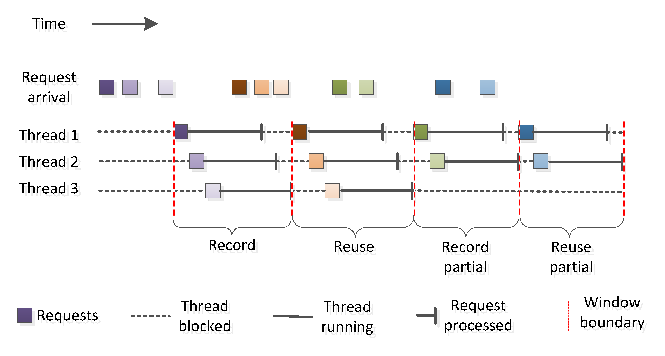
\includegraphics[width=0.7\linewidth]{peregrine/figures/window-idea}
\caption{{\em Recording and reusing schedules for a server program with
    three threads.}  The continuous execution stream is broken down into
  windows of requests, and \peregrine records and reuses schedules across
  windows.} \label{fig:window}
\end{figure}

Our observation is that server programs tend to return to the same
quiescent states, so \peregrine can use these states to split a continuous
request stream down to \emph{windows} of requests, as illustrated in
Figure~\ref{fig:window}.  Specifically, \peregrine buffers requests as they
arrive until it gathers enough requests to keep all worker threads busy.
It then runs the worker threads to process the requests, while buffering
newly arrived requests to avoid interference between windows.  If \peregrine
cannot gather enough requests before a predefined timeout, it proceeds
with the partial window to reduce response time.  By breaking a request
stream into windows, \peregrine can record and reuse schedules across
windows, stabilizing server programs.  
Server quiescent states may evolve.  For instance, a web server may cache
requests in memory.  Developers can annotate the functions that query
cache, and \peregrine treats the return values as inputs and selects proper
schedules.
Windowing reduces concurrency, but the cost is moderate based on our 
experiments.

\subsection{Evaluation} \label{sec:peregrine-eval}
We evaluated our \peregrine implementation on a diverse set of \nprog programs,
including \apache, a popular web server; \pbzip, a parallel compression
utility; \aget, a parallel \v{wget}-like utility; \pfscan, a parallel
\v{grep}-like utility; parallel implementations of 13
computation-intensive algorithms, 10 in \splash and 3 in \parsec; and
\racey, a benchmark specifically designed to exercise deterministic
execution and replay systems~\cite{racy-stress}.  All \splash benchmarks
were included except one that we cannot compile, one that our current prototype
cannot handle due to an implementation bug, and one that does not run
correctly in 64-bit environment.  The chosen \parsec benchmarks
(\blackscholes, \swaptions and \streamcluster) include the ones that (1)
we can compile, (2) use threads, and (3) use no x86 inline assemblies.
These programs were widely used in previous studies
(\eg,~\cite{lu:concurrency-bugs,syncfinder:osdi10,grace:oopsla09}).

In the remainder of this section, we focus on two questions:
\begin{enumerate}

\item Is \peregrine deterministic if there are
  data races?  Determinism is one of the strengths of \peregrine over the
  sync-schedule approach.

\item Is \peregrine fast?  For typical multithreaded
  programs that have rare data races, \peregrine should be roughly as fast as
  the sync-schedule approach.  Efficiency is one of the strengths of \peregrine
  over the mem-schedule approach.

\end{enumerate}

We evaluated \peregrine's determinism by checking whether \peregrine could
deterministically resolve races.  Table~\ref{tab:racy-edges} lists the seven
racy programs used in this experiment.  We selected the first five because
they were frequently used in previous
studies~\cite{avio:asplos06,ctrigger:asplos09,lu:concurrency-bugs,pres:sosp09}
and we could reproduce their races on our evaluation machine.  We selected the
integer flag race in \parsec to test whether \peregrine can handle ad hoc
synchronization~\cite{syncfinder:osdi10}.  We selected \racey to stress
test \peregrine: each run of \racey may have thousands of races, and if any of
these races is resolved differently, \racey's final output changes
with high probability~\cite{racy-stress}.

\begin{table}[t]
\small
\centering
\begin{tabular}{ccc}
{\bf Program} & {\bf Races} & {\bf Order Constraints} \\
\hline
\apache  & 0 & 0 \\
\pbzip   & 4 & 3 \\
\barnes  & 5 & 1 \\
\fft     & 10 & 4 \\
\lun      & 10 & 7 \\
\streamcluster & 0 & 0 \\
\racey   & 167974 & 9963 \\
\end{tabular}
\caption{{\em Hybrid schedule statistics.} Column {\bf Races} shows the
  number of races detected according the corresponding
  sync-schedule, and Column {\bf Order Constraints} shows the number of 
execution
  order constraints \peregrine adds to the final hybrid schedule.  The latter
  can be smaller than the former because \peregrine prunes subsumed execution
  order constraints~\cite{peregrine:sosp11}.  \peregrine detected no races for
  \apache and \streamcluster because the corresponding sync-schedules are
  sufficient to resolve the races deterministically; it thus adds no order
  constraints for these programs.} \label{tab:racy-edges}
\end{table}

For each program with races, we recorded an execution trace and computed a
hybrid schedule from the trace.  Table~\ref{tab:racy-edges} shows for each
program (1) the number of dynamic races detected according to the
sync-schedule and (2) the number of execution order constraints in the
hybrid schedule.  The reduction from the former to the latter shows how
effectively \peregrine can prune redundant order constraints~\cite{peregrine:sosp11}.
In particular, \peregrine prunes 94\% of the constraints
for \racey.  For \apache and
\streamcluster, their races are already resolved deterministically by
their sync-schedules, so \peregrine adds no execution order
constraints.

To verify that the hybrid schedules \peregrine computed are deterministic, we
first manually inspected the order constraints \peregrine added for each program
except \racey (because it has too many races for manual verification).  Our
inspection results show that these constraints are sufficient to resolve
the corresponding races.  We then re-ran each program including \racey 1000
times while enforcing the hybrid schedule and injecting delays; 
and verified that each run reused the schedule and computed equivalent results.
(We determined result equivalence by checking either the output or whether
the program crashed.)

\begin{figure}[t]
\centering
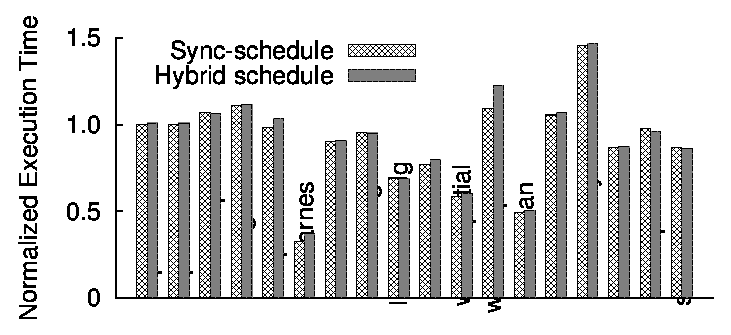
\includegraphics[width=0.7\columnwidth]{peregrine/figures/overhead}
\caption{{\em Normalized execution time when reusing sync-schedules
    v.s. hybrid schedules.}  A time value greater than 1
  indicates a slowdown compared to a nondeterministic execution without
  \peregrine.  We did not include \racey because it was not designed for
  performance benchmarking. } \label{fig:peregrine-overhead}
\end{figure}

Figure~\ref{fig:peregrine-overhead} shows the execution times when reusing hybrid
schedules; these times are normalized to the nondeterministic
execution time.  (The next paragraph compares these times to those of
sync-schedules.)  For \apache, we show the throughput (TPUT) and response
time (RESP).  All numbers reported were averaged over 500 runs.  \peregrine
has relatively high overhead on \watern (22.6\%) and \cholesky (46.6\%)
because these programs do a large number of mutex operations within tight 
loops. Still, this overhead is reasonable. Running \peregrine on these 
programs and workloads is below 46\%,
lower than the reported 1.2X-6X overhead of a mem-schedule \dmt
system~\cite{coredet:asplos10}.  Moreover, \peregrine speeds up \barnes, \lun,
\radix, \waters, and \ocean (by up to 68.7\%) because it safely skips
synchronization and sleep operations~\cite{cui:tern:osdi10}.  For the other
programs, \peregrine's overhead or speedup is within 15\%.  (Note that
increasing the page or file sizes of the workload
tends to reduce \peregrine's relative overhead
because the network and disk latencies dwarf \peregrine's.)

